\section{Introducción y Motivación}

% ==============================================
\begin{frame}{Vehículos Autónomos}
	\begin{itemize}
		\item Los vehículos autónomos no cuentan con una tripulación ni un piloto a bordo. Estos son comandados de forma remota, o bien tienen la capacidad de hacerlo por sí solos.
		\item Gran variedad de sensores + computadora central = sistema de navegación y reconocimiento del entorno.
	\end{itemize}
	\begin{center}
		\resizebox{\textwidth}{!}{%
			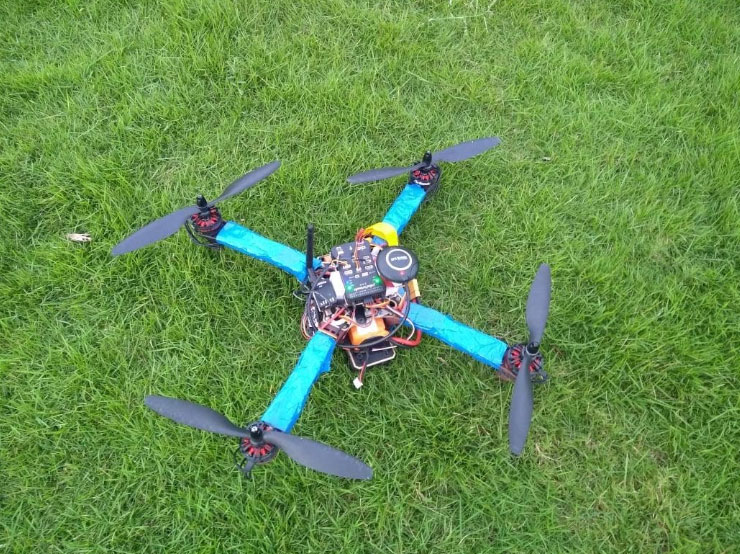
\includegraphics[height=3cm]{img/uav_2.jpg}%
			\quad
			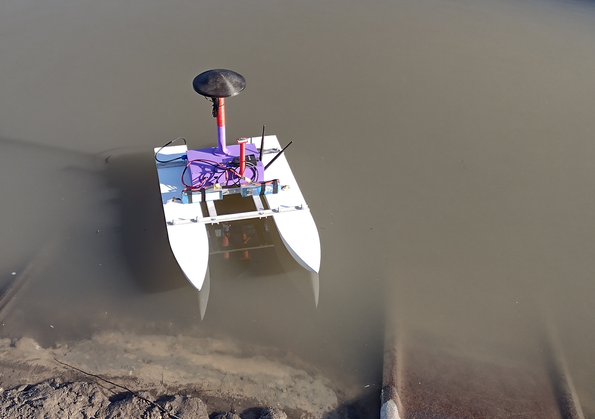
\includegraphics[height=3cm]{img/ASV_leo.png}%
			\quad
			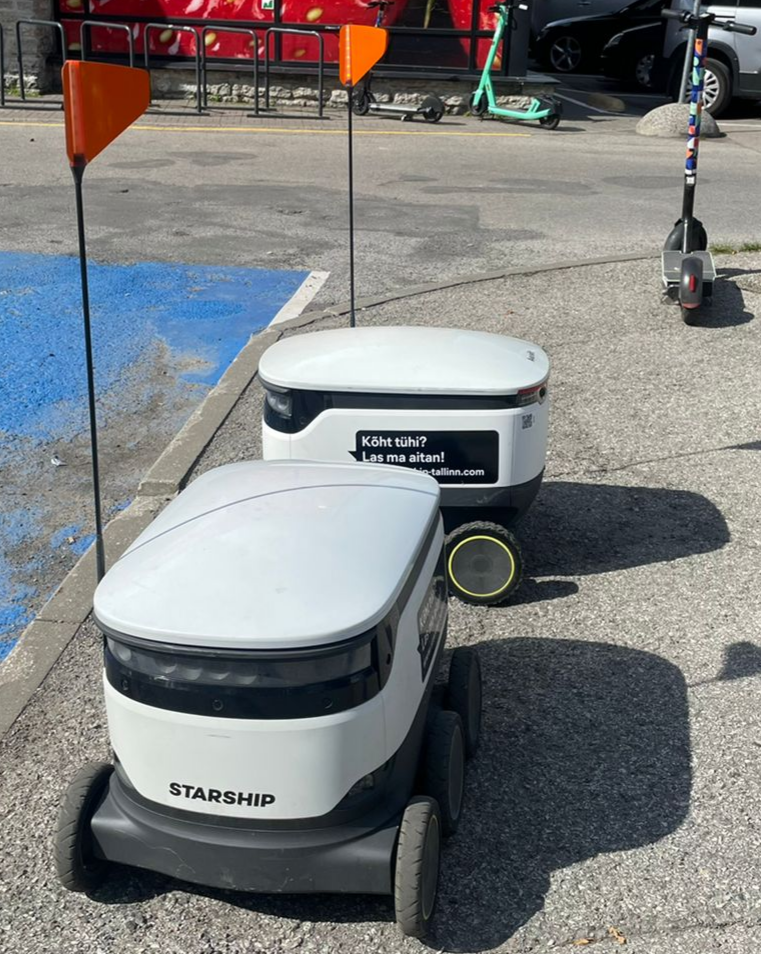
\includegraphics[height=3cm]{img/movil_robot.png}%
		}
	\end{center}
\end{frame}

\begin{frame}{Vehículos Autónomos}
	\begin{columns}
    \column{0.5\textwidth}
        \begin{itemize}
            \item Originalmente desarrollados para uso en aplicaciones militares.
            \item Desarrollo y mantenimiento menos costoso frente a vehículos tripulados.
            \item Motivación: Realizar tareas que de otra forma pondrían en riesgo a la tripulación.
        \end{itemize}
    \column{0.5\textwidth}
            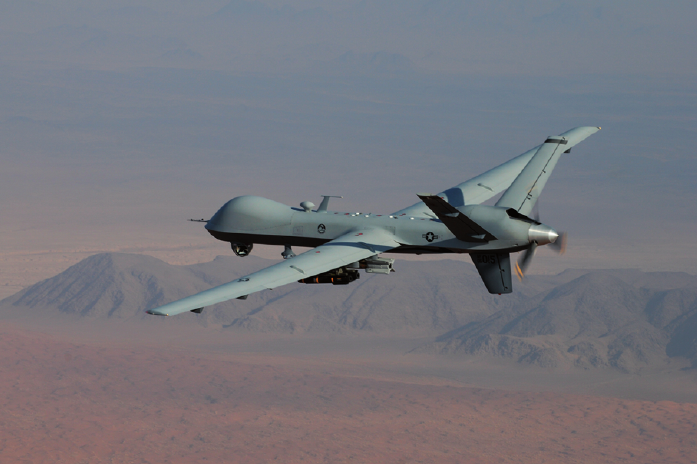
\includegraphics[width=\textwidth]{img/dron_militar_1}
	\end{columns}
\end{frame}

\begin{frame}{Vehículos Autónomos}
	% \begin{columns}
	% \column{0.5\textwidth}
	%     \includegraphics[width=4cm]{img/drones_sar_todo.png}
	%     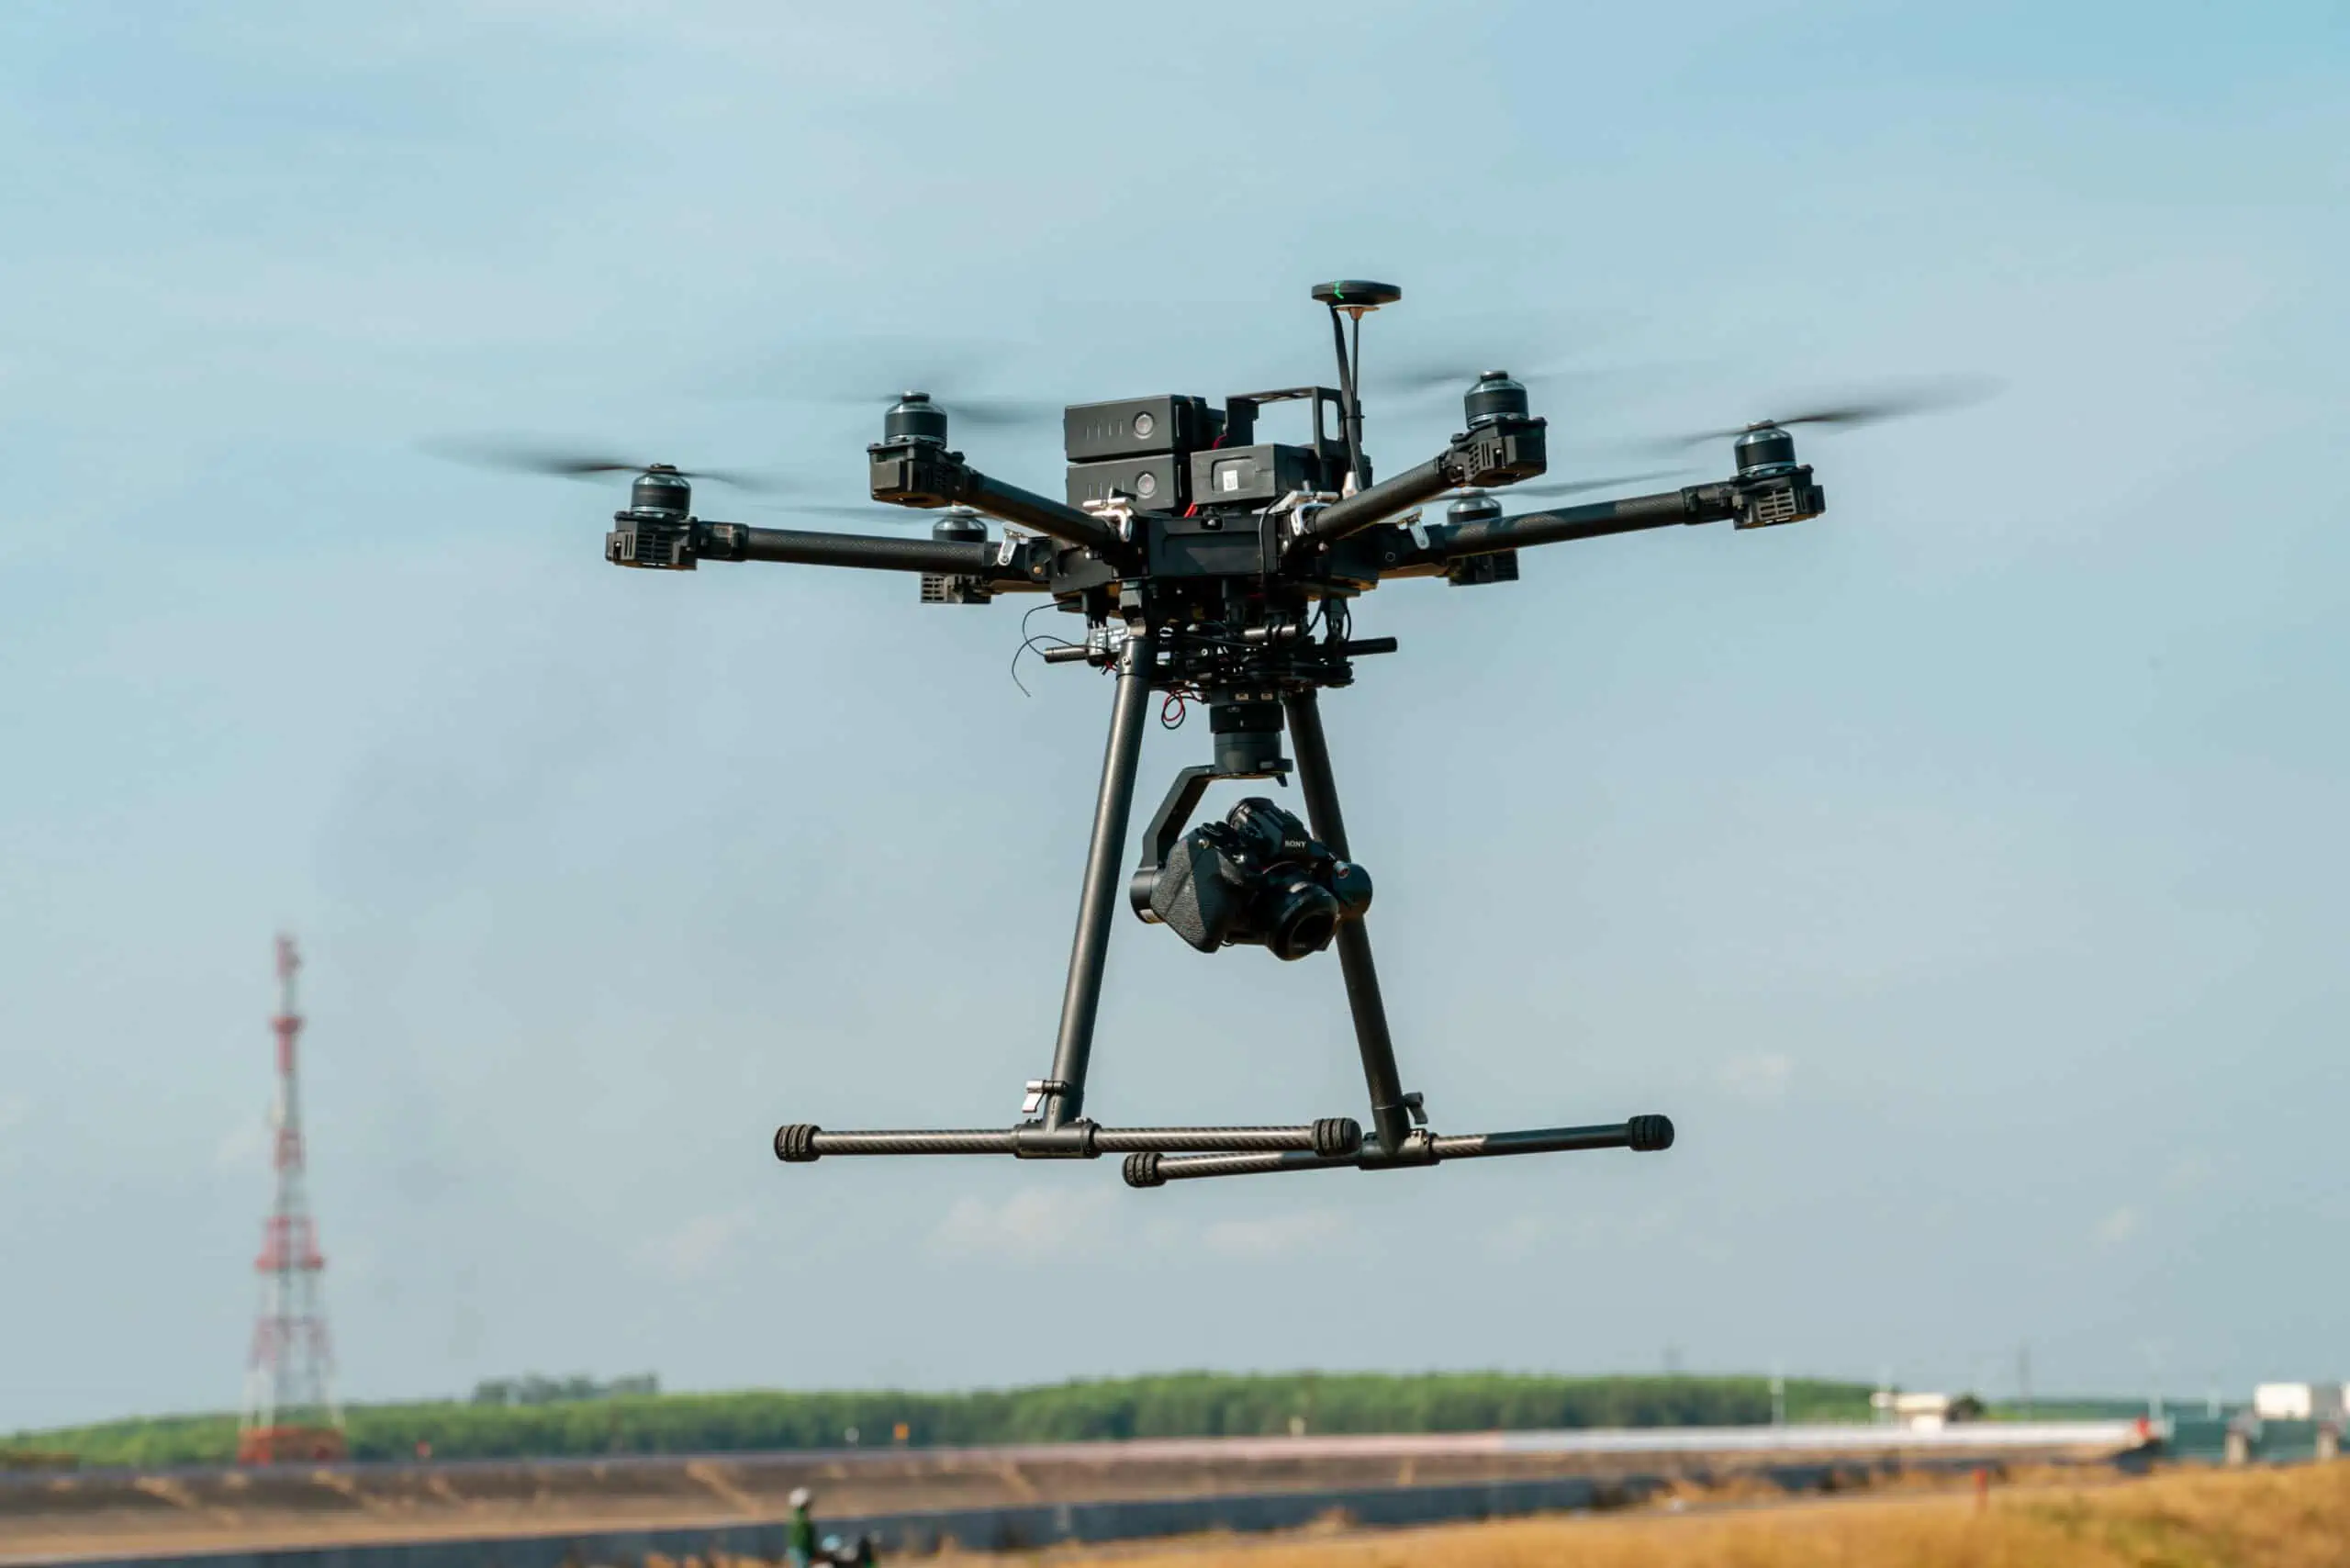
\includegraphics[width=4cm]{img/drone_camer.png}
	% \column{0.5\textwidth}
	% 	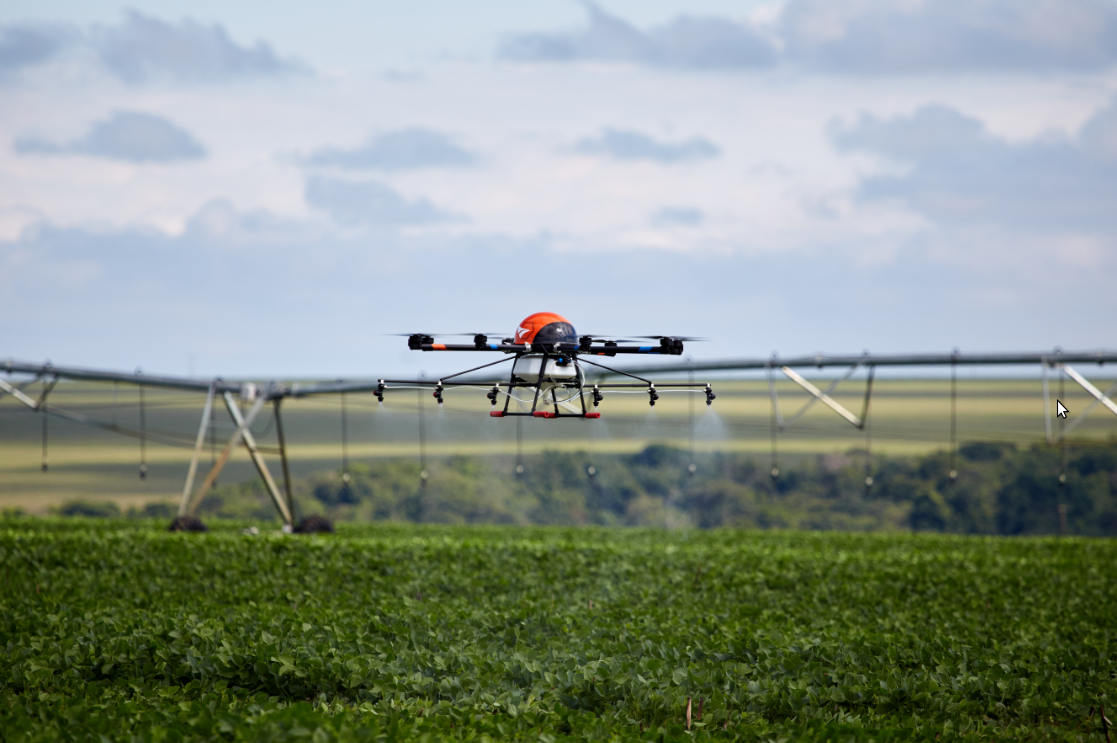
\includegraphics[width=4cm]{img/drone_agricultura.png}
	%     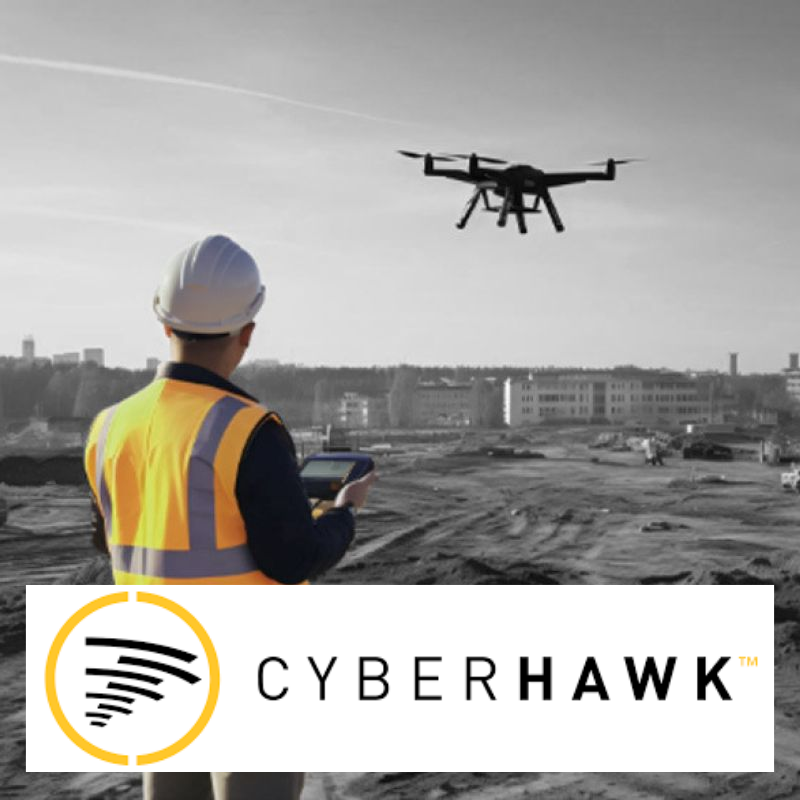
\includegraphics[width=4cm]{img/inspeccion_completo.png}
    % \end{columns}
    % \makebox[\textwidth]{%
	% \begin{minipage}{1\textwidth} % <--- can be as large the slide size permits
	% 	\includegraphics[width=.3\textwidth,keepaspectratio]{img/drones_sar_todo.png}\hfill%
	% 	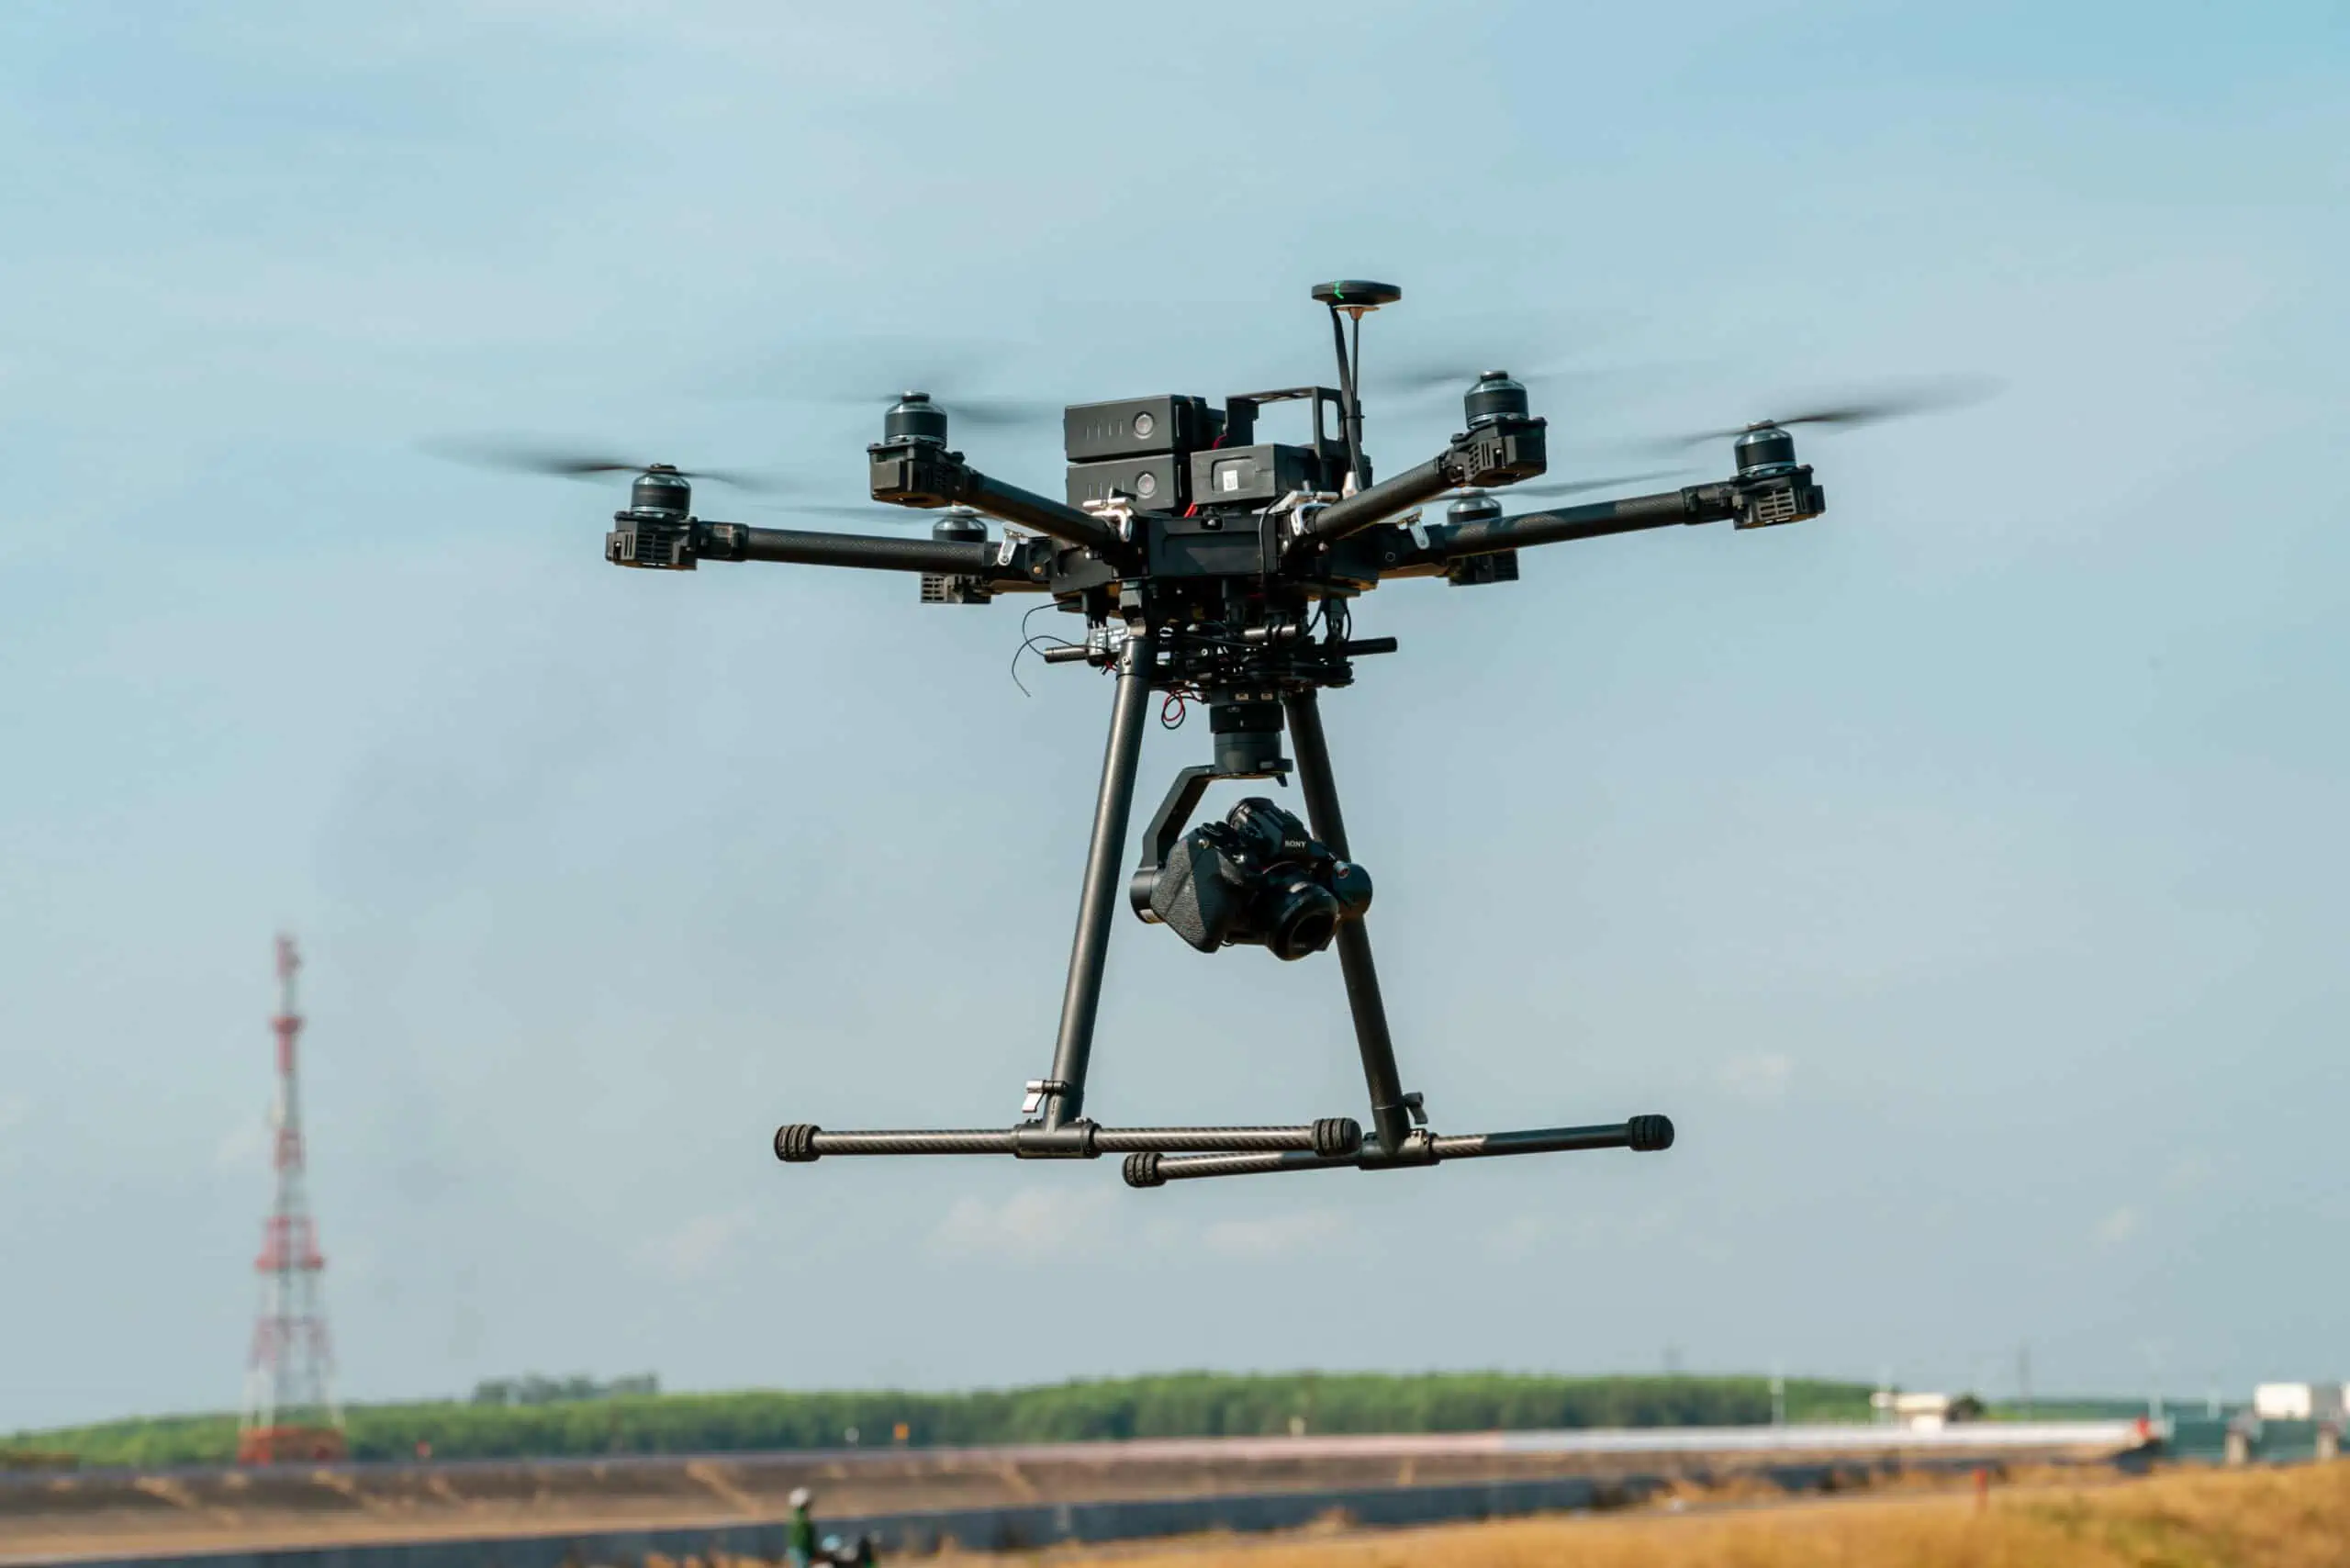
\includegraphics[width=.3\textwidth,keepaspectratio]{img/drone_camer.png}\\[4pt]
	% 	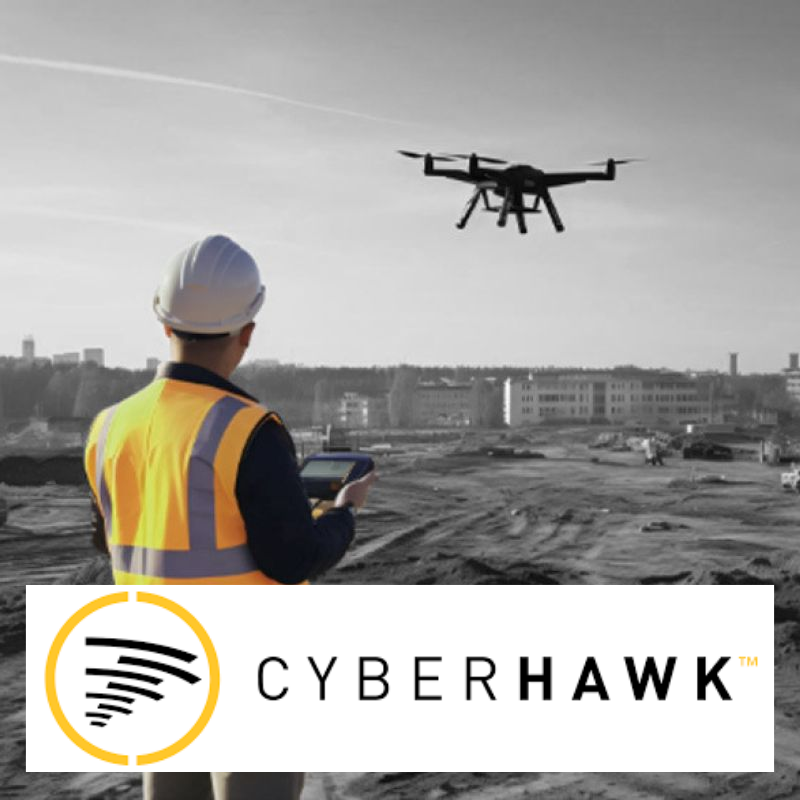
\includegraphics[width=.3\textwidth,keepaspectratio]{img/inspeccion_completo.png}\hfill%
	% 	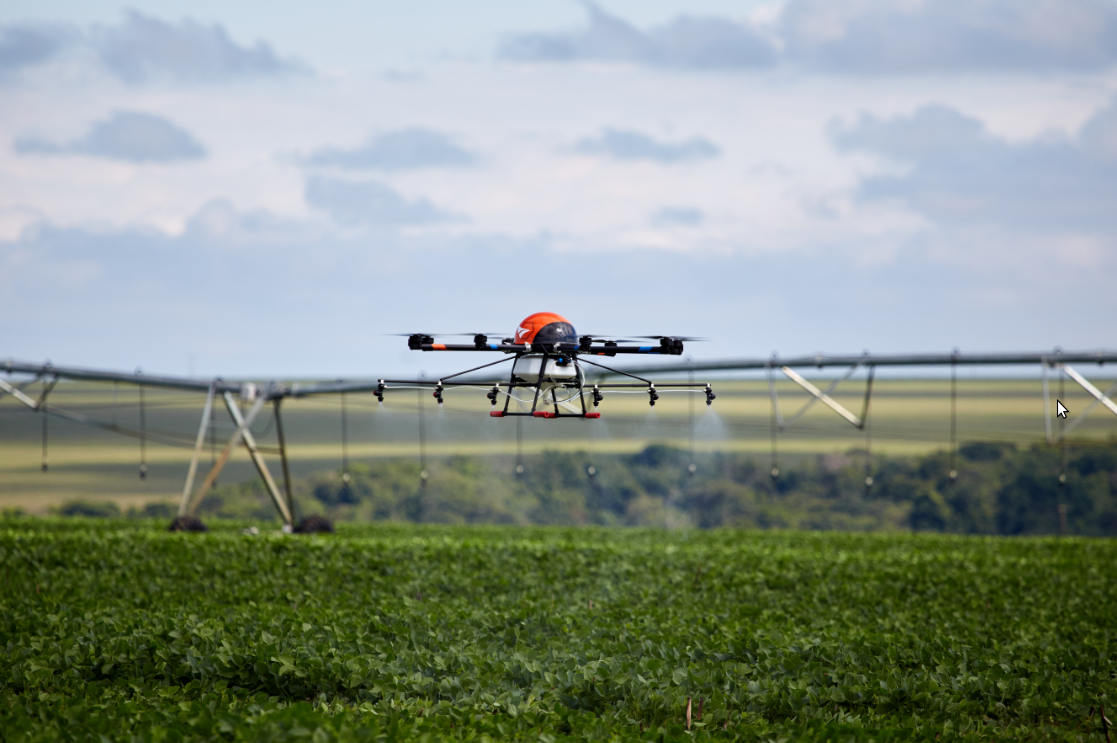
\includegraphics[width=.3\textwidth,keepaspectratio]{img/drone_agricultura.png}
	% 	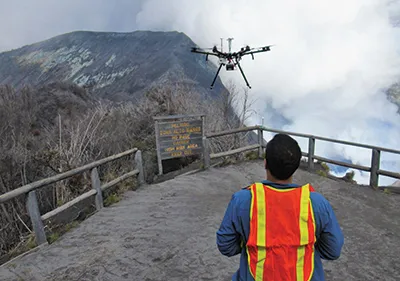
\includegraphics[width=.3\textwidth,keepaspectratio]{img/drone_volcano.png}
	% 	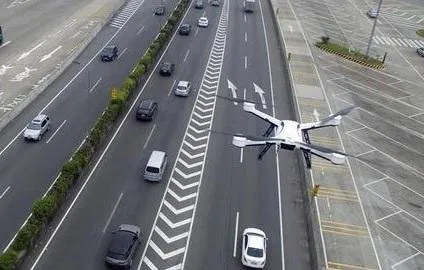
\includegraphics[width=.3\textwidth,keepaspectratio]{img/drone_traffic.png}
	% \end{minipage}
	\makebox[\textwidth]{%
	\begin{minipage}{1\textwidth} % <--- can be as large the slide size permits
		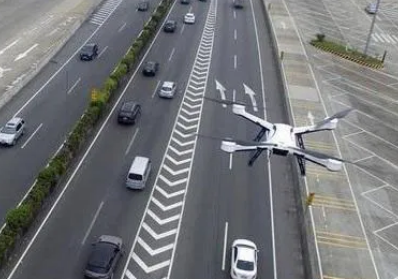
\includegraphics[height=.35\textheight,keepaspectratio]{img/drone_traffic_size.png}\hfill
		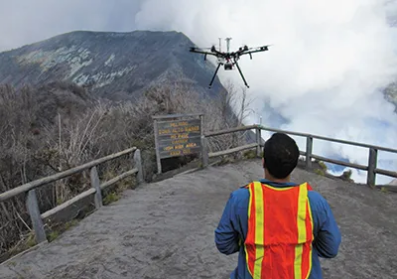
\includegraphics[height=.35\textheight,keepaspectratio]{img/drone_volcano_size.png}\hfill
		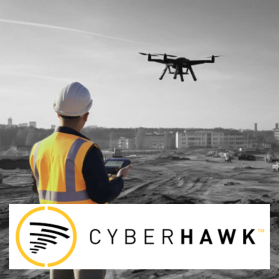
\includegraphics[height=.35\textheight,keepaspectratio]{img/drone_inspeccion_size.png}\\[20pt]
		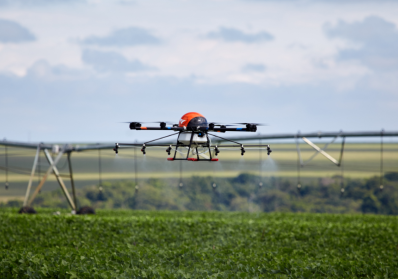
\includegraphics[height=.35\textheight,keepaspectratio]{img/drone_agricultura_size.png}\hfill
		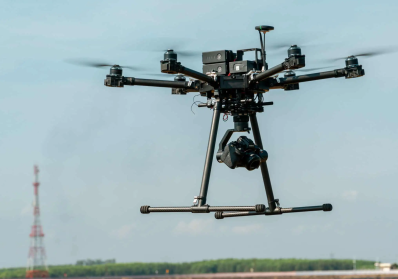
\includegraphics[height=.35\textheight,keepaspectratio]{img/drone_camera_size.png}\hfill
		
\includegraphics[height=.35\textheight,keepaspectratio]{img/drones_sar_size.png}
	\end{minipage}
}
\end{frame}

\begin{frame}{Vehículos Autónomos}
	\begin{itemize}
		\item Cada vez tienen mayor presencia en zonas civiles.
		\item La incorporación de drones permite realizar tareas costosas,  riesgosas o críticas de forma segura.
		\item Teniendo esto en cuenta, la confiabilidad es un aspecto que toma mayor relevancia.
		\item {COMPLETAR CON EJEMPLOS DE ACCIDENTES DE DRONES}
	\end{itemize}
\end{frame}

% ==============================================
\begin{frame}{Computadora de Vuelo}
	\begin{columns}
		\column{0.39\textwidth}
		\begin{itemize}
			\item <1->Los drones se componen de varios elementos.
			\item <3->Todos ellos son susceptible de manifestar fallas.
			\item <4->En este trabajo se abordan aspectos relacionados a la \textbf{computadora de vuelo}.
		\end{itemize}
		\column{0.6\textwidth}
			\begin{overprint}
				\onslide<2>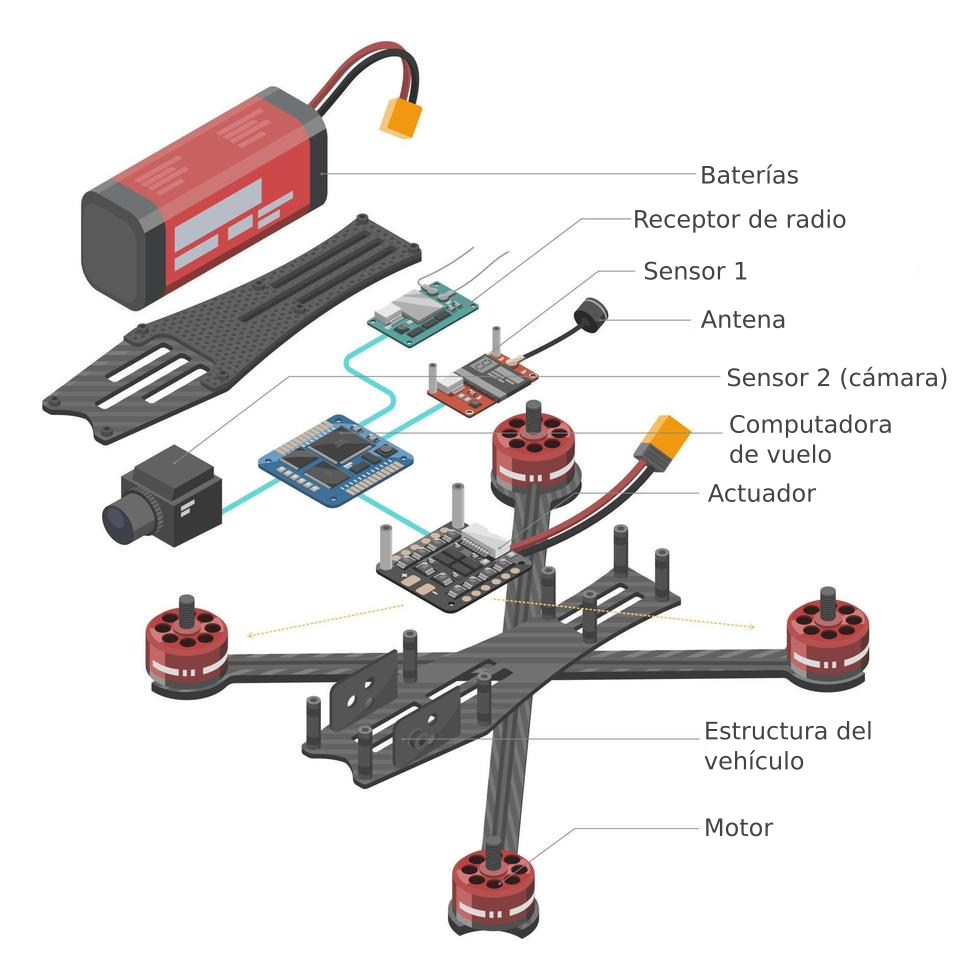
\includegraphics[width=\textwidth]{img/partes_de_un_drone.png}
				\onslide<3>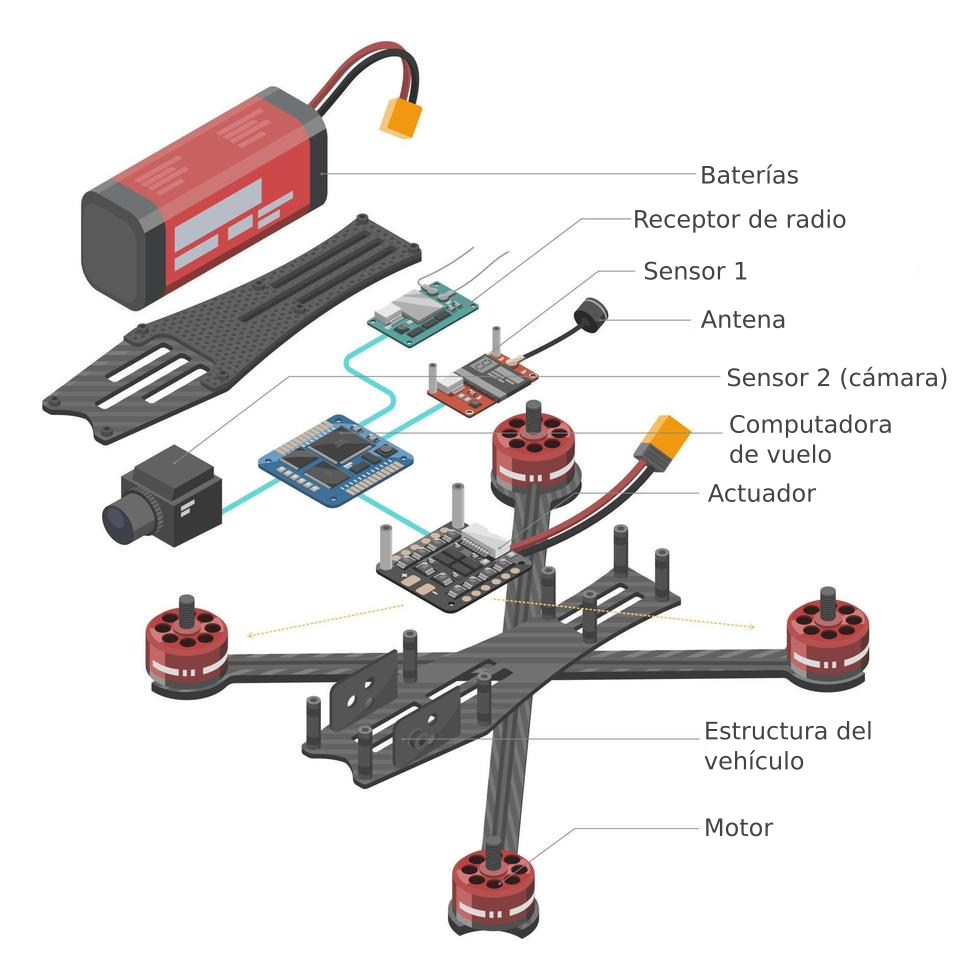
\includegraphics[width=\textwidth]{img/partes_de_un_drone.png}
				\onslide<4>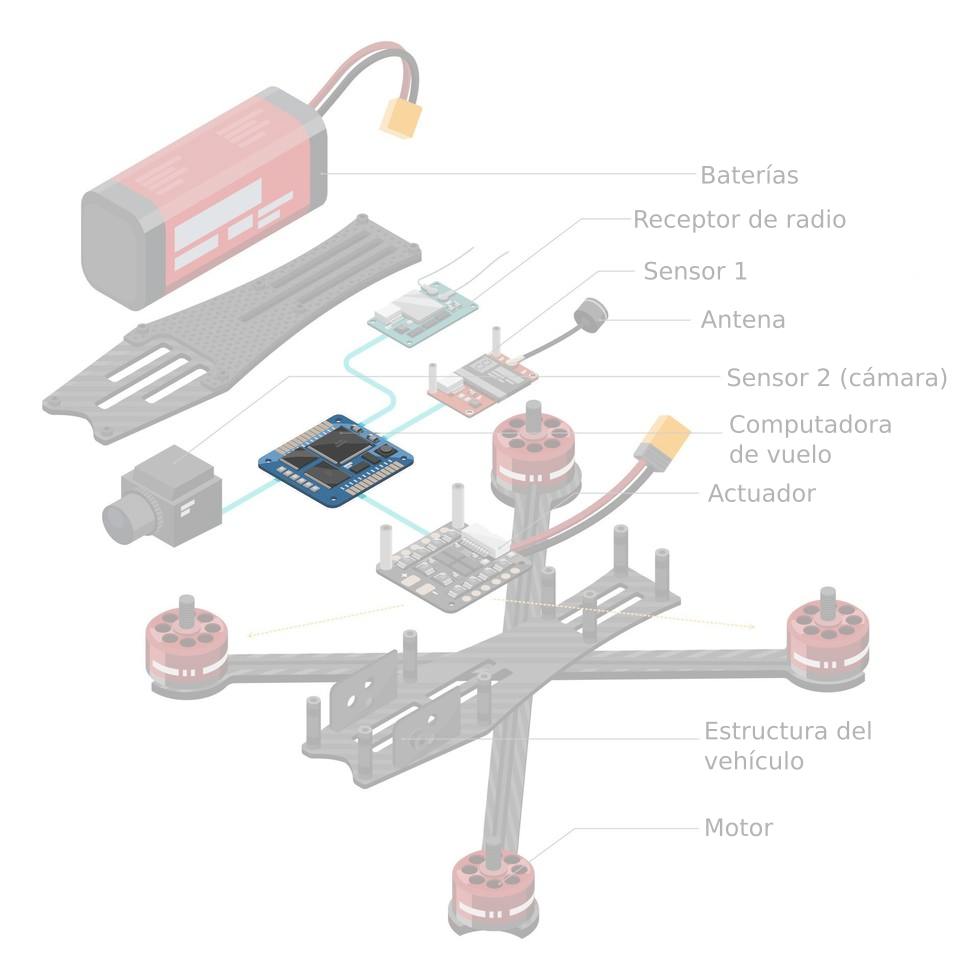
\includegraphics[width=\textwidth]{img/partes_de_un_drone_transparencia.png}
			\end{overprint}
	\end{columns}
\end{frame}

\begin{frame}{Computadora de Vuelo}

\end{frame}

\begin{frame}{Vehículos Autónomos}
	\begin{itemize}
		%\item Teniendo en cuenta la relevancia que han tomado en zonas civiles, resulta mandatorio asegurar cierto grado de confiabilidad en su funcionamiento.
		\item Cada vez tienen mayor presencia en zonas civiles.
		\item La incorporación de drones permite realizar tareas costosas,  riesgosas o críticas de forma segura.
		\item Teniendo esto en cuenta, la \textbf{confiabilidad} es un aspecto que toma mayor relevancia.
	\end{itemize}
    \begin{block}{Confiabilidad}
    	Probabilidad de que un sistema pueda cumplir con su función de manera correcta en un intervalo de tiempo $\left[t_0;t\right]$, dado que sí podía hacerlo en $t_0$.
    \end{block}
    \begin{columns}
    	\column{0.4\textwidth}
			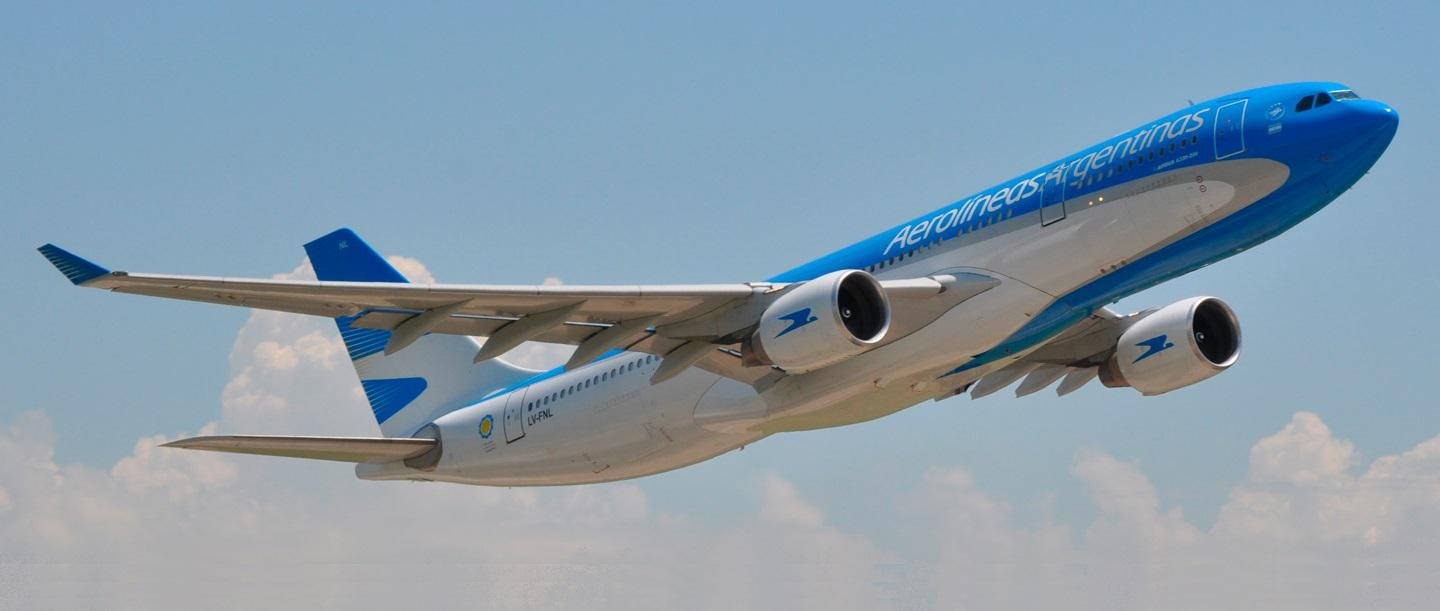
\includegraphics[width=\textwidth]{img/avion_comercial.jpg}
    	\column{0.6\textwidth}
            \begin{itemize}
            	\item El aspecto más importante en aviones comerciales: $10^{-9}/h$ de vuelo.
            	\item Aviones militares: $10^{-7}/h$ de vuelo.
            	\item Drones militares: $10^{-5}/h$ de vuelo.
            	\item ¿\underline{Drones civiles/comerciales}?
            \end{itemize}
    \end{columns}
\end{frame}

